\section{Background and Related Work}
\label{sec:background}

FPGAs (Field Programmable Gate Array Logic) are applied in sequence comparison in Large Sequence databanks for the reason that they significantly improve performance due to parallel architecture. There are number of proposed and applied implementations of BLAST algorithm on FPGA in order to address the issue of biological sequence alignment [*1]. Examples of proposed hardware implementations can be Mercury BLASTn [*2], Mercury BLASTp [*4], Tree-BLAST [*5], RC-BLAST [*6], FPGA/FLASH Accelerator [*3], Multiengine BLASTn Accelerator  [*7]. 
//
The architectures mentioned above are based on the Word Position Record-Based Search (WPRBS) method[*8], which stores words of query sequence in a constructed storage table and compares the subject sequence with storage table to detect the hit. The strategy is widely applied; however performance and searching capacity limitations are still extant. The reason is that during one clock cycle only one word can be searched, and thus more than one hit per clock cycle cannot be detected. Timing issue is also caused by shortage in WPRBS searching capacity due to limited number of memory ports in FPGAs.
//
Examples of such architecture are Mercury BLASTn [*2] and Mitrion [*9]. In these two systems storage tables are stored in the external memory SRAM that is attached to the FPGA, since the tables storing the words of long query sequences will require vast amount of space in internal memory RAM. Searching is performed by comparing one subject sequence from database to every word in the storage table simultaneously during one clock cycle. Apparently, performance of the system will be low: accessing external memory SRAM for getting subject sequence from database every time consumes significant amount of time.    
//     
Performance could be improved by FPGA/FLASH [*3], which minimizes accesses to the external memory by enabling to detect several exact hits simultaneously. It is due to index structure of the database: words in the sequence associated with their position in the database and neighboring elements. However, huge space in the memory is needed to store index of the database as well as database itself. For database exponentially growing every year this architecture will not be efficient. 
//
In order to solve the timing isuse, the architecture Multiengines BLASTn [*7] is constructed in such way that compares 64 subject sequences simultaneously due to its 64 identical computing units. The architectures described above are based on WPRBS.
//
There is another method based on systolic array that does not construct tables. Needleman-Wunsch algorithm [*10] and dynamic programming algorithm that apply systolic array was implemented on SPLASH2 by D. Hoang et. al. [*11], [*12]. Another algorithm that uses systolic array called Smith Waterman matching algorithm was implemented by S. Guccione et. al. [*13], also at Virginia Tech [*14] and Nanyang Techological University [*15]. 

\begin{figure}
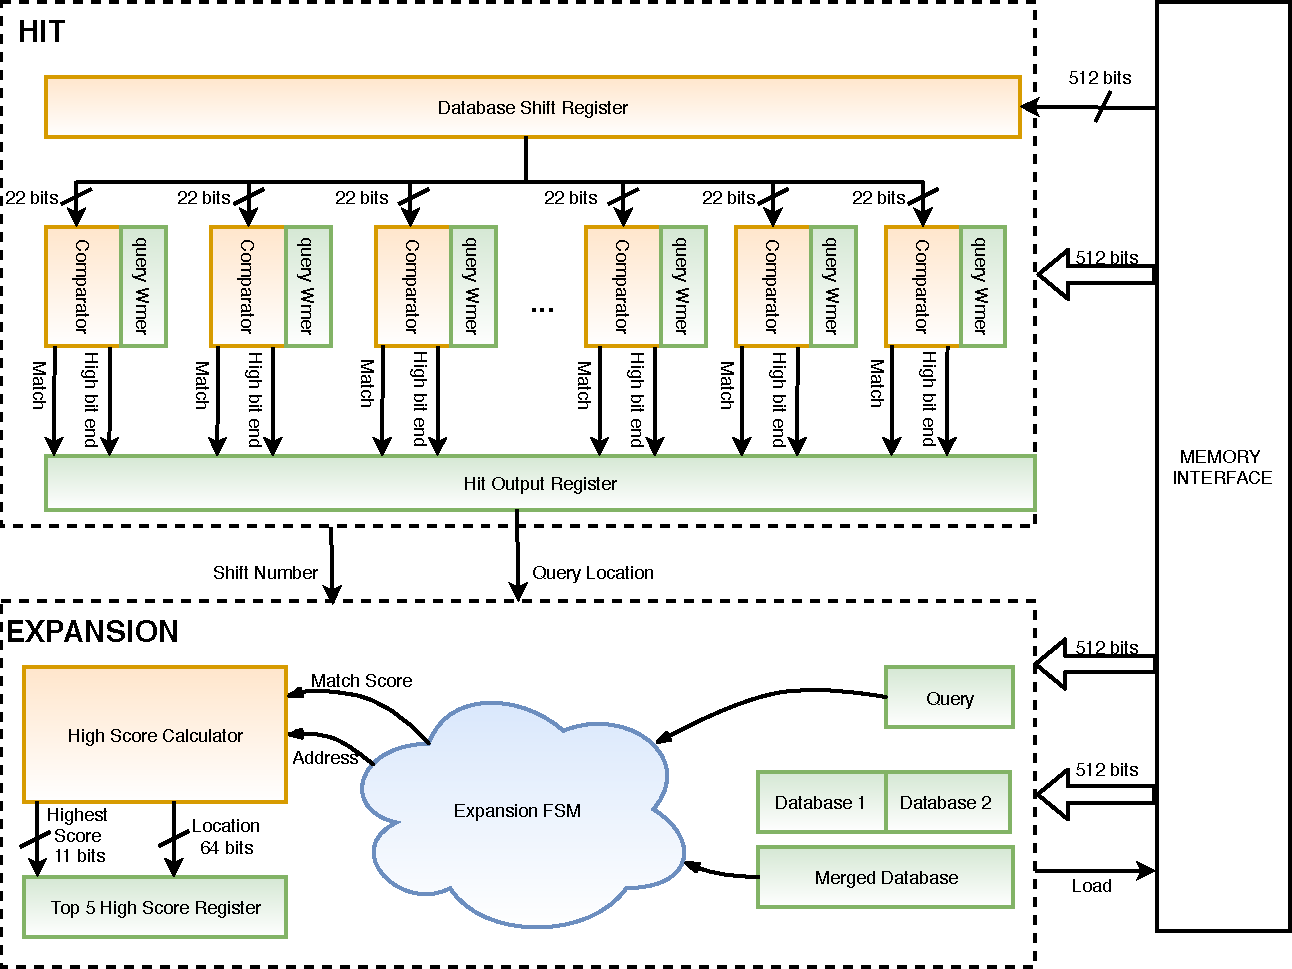
\includegraphics[width=\textwidth]{Figures/BlastMachine.pdf}
\caption{A figure caption is always placed below the illustration.
Please note that short captions are centered, while long ones are
justified by the macro package automatically.} \label{fig1}
\end{figure}


In paper \cite{vipin2019}

adfsadffasdf
